\documentclass[12pt,ebook]{../notes}
\usepackage{docmute}
\graphicspath{{img/}}
\title{Конспект по анализу за 3 семестр}
\date{\today}

\author{Лектор: А.~А.~Лодкин \\
Записал :\texttt{ta\lower 0.1em \hbox{x}us}}

\begin{document}
 
\maketitle
\tableofcontents
\clearpage

\chapter{Анализ в \texorpdfstring{$\R^n$}{}}
%------------------------------------------------------------
% Description : Calculus in \R^n space
% Author      : taxus-d <iliya.t@mail.ru>
% Created at  : ??? 
%------------------------------------------------------------
\documentclass[12pt,trimbord]{../../../notes}
\usepackage{silence}
\WarningFilter{latex}{Reference}
\graphicspath{{../../img/}}

\begin{document}

\paragraph{Оценка приращения дифференциального отображения}
\label{par:diffspace::diffestim}

\begin{prop}\label{prop:diffspace::diffestim::lagrfail}
  Пусть $f\colon \R^n \to \R^m$, $m \geqslant 2$. Тогда формула Лагранжа
  \[
    f(b) - f(a) = f'(c)(b - a)
  \]
  не работает.
\end{prop}
\begin{exmp*}\label{exmp:diffspace::diffestim::lagrfail}
  Пусть 
  \[
    f(t) := (\cos t, \sin t), b - a = 2\pi
  \]
\end{exmp*}

\begin{thrm}[об оценке приращения отображения]\label{thrm:diffspace::diffestim::diffestim}
  Пусть $f\colon G \subset \R^n \to \R^m$, $G$~--- выпуклое, $f$~--- дифференцируема, 
  \[ 
    \forall\, x \in G \;\: \| f'(x) \| \leqslant M 
  \]
  Тогда $\forall\, a,b \in G \;\: \|f(b) - f(a)\| \leqslant M \| b-a \|$
\end{thrm}

\begin{ittproof}
  <<Окружим>>  исходную функцию:
  \[
    F = \psi \circ f \circ \varphi
  \]
  где 
  \begin{align*}
    \varphi&: \R^n \to \R^m & \varphi(t) &:= t(b-a) + a, & t&\in [0,1] \\
    \psi&: \R^m \to \R & \psi(y) &:= \langle y, \ell \rangle, & \ell &= f(b)-f(a) 
  \end{align*}
  Заметим, что $F$~--- обычная вещественнозначная функция. Так что для неё работает формула
  Лагранжа:
  \[
    \exists\, c \in [0,1] \colon F(1)-F(0) = F'(c)(1-0) = F'(c)
  \]
  Тогда из свойств нормы (по ходу дела обозначим $\varphi(c)$ за $x$):
  \[
    \|F'(c)\| = \|\psi'(f(x)) \cdot f'(x) \cdot \varphi'(c)\| \leqslant 
    \|\psi'(f(x)) \| \cdot \| f'(x) \| \cdot \| \varphi'(c)\|
  \]
  Здесь тонкость в обозначениях. Производные~--- вроде матрицы, поэтому их нормы~--- что-то
  странное на первый взгляд. На самом деле смысл немного иной. 
  \[
    \mathrm d L(x, h) = f'(x) \cdot h
  \]
  Таким образом, дифференциал~--- неплохое линейное отображение. А под <<нормой производной>>
  имеется в виду норма соответствующего линейного отображения.

  Теперь давайте что-нибудь скажем про эти нормы. 
  \begin{enumerate}
    \item $\varphi'(t) = (b-a) \Rightarrow \| \varphi'(c) \| = \| b - a\|$
    \item $\psi(y) = \langle y, l \rangle$, $\| \psi\| = \|\ell\|$      
  \end{enumerate}
  Так что 
  \[
    \| F'(c)\| \leqslant M \cdot \| \ell \| \cdot \|b-a\|
  \]
  С другой стороны:
  \[
    F(1) - F(0) = \psi(f(b)) - \psi(f(a)) = \langle f(b), \ell \rangle - \langle f(a), \ell \rangle
    = \langle \ell, \ell \rangle  = \|\ell \|^2
  \]
  В итоге, совмещая оба выражения, приходим к утверждению теоремы.
\end{ittproof}

\paragraph{Частные производные высших порядков}
\label{par:diffspace::highpartial}

\begin{defn}\label{defn:diffspace::highpartial}
  Пусть $f \colon G \subset \R^n \to \R$, существуют производные $k$-го порядка. Тогда
  \[
    \partial_{i_1, \dotsc, i_{k+1}}^{k+1} f(x) := \partial_{i_{k+1}}(\partial^k_{i_1, \dotsc, i_{k+1}} f) (x)
  \]
\end{defn}
\begin{rem}\label{rem:diffspace::highpartial::smooth}
  $C^p(G)$~--- класс функций, определённых в $G$ с непрерывной производной до $p$-го порядка
  включительно.
  Функции из $C^1$ ещё называются гладкими.
\end{rem}

\begin{thrm}[Зависимость производных $p$-го порядка от перестановки переменных]
  \label{thrm:diffspace::highpartial::permut}
  Пусть \mbox{$f \in C^p(G)$}, $x\in G$. При этом
  \[
    \begin{split}
      i &= \{ i_1, \dotsc, i_p \mid i_k \in \{1, \dotsc, n\}\} \\
      j &= \{ j_1, \dotsc, j_p \mid j_k \in \{1, \dotsc, n\}\} \\
      j &= \pi(i)
    \end{split}
  \]
  Тогда 
  $\partial_i^{\,p} f(x) = \partial_j^{\,p} f(x)$
\end{thrm}
\begin{rem}\label{rem:diffspace::highpartial::permut}
  Тут важно, что есть целая окрестность. Одной точки не хватит.
\end{rem}

\paragraph{<<Многомерный>> дифференциал высоких порядков}
\label{par:diffspace::highdiff}

\begin{defn}\label{defn:diffspace::highdiff}
  Пусть $f \colon G \subset \R^n \to \R$, $f\in C^p(G)$
  \[  
    \del^p f(x) := \sum_{1 \leqslant i_1 \leqslant \dotsb \leqslant i_p \leqslant n}
    \frac{\partial^p f}{\partial x_{i_p} \dotso \partial x_{i_p}} \, \del x_{i_1} \dotsm \del x_{i_p}
  \]
\end{defn}

\begin{stat}\label{stat:diffspace::highdiff::binom}
  Если частные производные можно переставлять, то
  \[
    \del^p f(x) = \sum_{\substack{\alpha_i \geqslant 0 \\ \sum \alpha_i = p}} 
    \frac{p!}{\alpha_1! \dotsm \alpha_n!} \, 
    \frac{\partial^p f}{\partial x_1^{\alpha_1}\dotso \partial x_n} \,\del x_{i_1} \dotsm \del x_{i_p}
  \]
\end{stat}

\paragraph{Формула Тейлора для функций многих переменных}
\label{par:diffspace::taylor}

\begin{thrm}\label{thrm:diffspace::taylor}
  Пусть $f \in C^p(G), G\in \R^n$, $a\in G$. Пусть также $h\in \R^n \colon a+h \in G$.
  Тогда 
  \[
    f(a+h) = \sum_{k=0}^p \frac{1}{k!} \, \del^k f(a,h) + R_p(h)
  \]
  Остаток $R_p(h)$ можно представить несколькими способами:
  \begin{enumerate}
    \item В форме Пеано: $R_p(h) = o(\|h\|^p)$
    \item В форме Лагранжа: $R_p(h) = \dfrac{1}{(p+1)!}\, \del^{p+1} f(a + \theta h, h)$, 
      $\theta \in (0,1)$
  \end{enumerate}

\end{thrm}

\paragraph{Экстремумы}
\label{par:diffspace::extrema}

\begin{defn}\label{defn:diffspace::extrema}
  Пусть $f\colon G \subset \R^n \to \R$, $a\in G$. Тогда говорят, что $f$ имеет в $a$ максимум (нестрогий), если
  \[
    \exists\, U(a) \colon \forall\, x \in U \;\: f(x) \leqslant f(a)
  \]
  Когда неравенство строгое, а окрестность проколотая, то максимум~--- строгий
  Для минимума нужно $\geqslant$.
\end{defn}

\begin{thrm}[Необходимое условие экстремума]\label{thrm:diffspace::extrema::ness}
  Пусть $a$ внутренняя точка $G \subset \R^n$, $f\in C^1(a)$. Тогда если $f$ имеет в $a$ экстремум, то
  \[
    \del f(a) = 0 \Leftrightarrow \forall\,i \;\: \partial_i f(a) = 0
  \]
\end{thrm}

\begin{thrm}[Необходимое условие экстремума]\label{thrm:diffspace::extrema::suff}
  Пусть $a\in G \subset \R^n$, $a$~--- внутренняя точка, $f\in C^2(a)$.
  \begin{enumerate}
    \item $\del f(a) = 0$, $\del^2 f(a) > 0 \Rightarrow$ $f$ имеет в $a$ $\min$
    \item $\del f(a) = 0$, $\del^2 f(a) < 0 \Rightarrow$ $f$ имеет в $a$ $\max$
    \item $\del f(a) = 0$, $\del^2 f(a) \lessgtr 0 \Rightarrow$ ничего нет
    \item $\del f(a) = 0$, $\del^2 f(a) \leqslant 0 \Rightarrow$ $f$ не имеет в $a$ $\min$
    \item $\del f(a) = 0$, $\del^2 f(a) \geqslant 0 \Rightarrow$ $f$ не имеет в $a$ $\max$
  \end{enumerate}
\end{thrm}

\paragraph{Понятие о неявной функции}
\label{par:diffspace::implicit2}

\begin{defn}\label{defn:diffspace::implicit2}
  Пусть $F\colon G \subset \R^2 \to \R$. Рассмотрим уравнение
  \begin{equation}
    \label{eq:diffspace::implicit2::base}
    F(x, y) = 0
  \end{equation}

  Пусть $a =(x_0, y_0)$ удовлетворяет \eqref{eq:diffspace::implicit2::base}, 
  а $U$~--- окрестность $a \colon$ $U = U_x \times U_y$.
  Тогда будем говорить, что уравнение \eqref{eq:diffspace::implicit2::base} определяет неявную 
  функцию $f$ в $U$, если
  \[
    \forall\, x\in P \; \exists!\, y\in Q \colon F(x,y) = 0 \hspace{1.5em} (y = f(x))
  \]
\end{defn}

\begin{thrm}[О неявной функции]\label{thrm:diffspace::implicit2}
  Пусть $F\colon G\subset \R^2 \to \R$, $F\in C^1(x_0,y_0)$, а $a=(x_0, y_0) \colon$
  \begin{enumerate}
    \item $F(x_0, y_0) = 0$
    \item $F_y'(x_0, y_0) \neq 0$
  \end{enumerate}
  Тогда 
  $\exists\, P(x_0), Q(y_0) \colon $ в $U = P\times Q$ уравнение \eqref{eq:diffspace::implicit2::base} 
  задаёт неявную функцию $f\colon P\to Q$. При этом
  \[
    f\in C^1 \land f'(x) = - \frac{F_x'(x,y)}{F_y'(x,y)}
  \]
\end{thrm}
\begin{ittproof}
  \begin{enumerate}
    \item (Доказательство существования) \\
      Рассмотрим $\varphi(y) = F(x_0, y)$. Пусть НУО $F_y'(x_0, y_0) > 0$.
      Тогда 
      \[
        \exists\, U_\varepsilon(x_0, y_0) \colon \forall\, x, y \in U \;\: F_y'(x, y) > 0
      \]
      Обозначим соответствующие проекции $U$ (шар) на координатные оси за $U_x, U_y$
      Получается, что $\varphi \uparrow U_y = (y_0 - \varepsilon; y_0 + \varepsilon)$.
      Тогда 
      \[
        \begin{split}
          \exists\, V_1(x_0) &\colon \forall\, x\in V_1 F(x, y+\varepsilon) > 0 \\
          \exists\, V_2(x_0) &\colon \forall\, x\in V_2 F(x, y-\varepsilon) < 0 \\
                           P &= V_1 \cap V_2
        \end{split}
      \]
      Тогда из теоремы Больцано-Коши и монотонности $\varphi$
      \[
        \forall\, x \in P \; \exists!\, y\in Q=U_y \colon F(x, y) = 0
      \]
      В итоге получилось определение неявной функции.
    \item Непрерывность в $(x_0, y_0)$ вроде очевидна, мы же каждому $x$ из $P$ сопоставили 1
      $y$ из $Q$. Принадлежность классу $C$ можно установить проведя аналогичные рассуждения
      для $x\in P(x_0)$
    \item С гладкостью что-то странное. Можно наверное сделать как в Зориче.
    \item $F(x, f(x)) \equiv 0 \Rightarrow F_x'\cdot 1 + F_2'f'(x) = 0$
  \end{enumerate}
\end{ittproof}

\paragraph{Полнота пространства \texorpdfstring{$\R^n$}{}}
\label{par:diffspace::banach}

\paragraph{Теорема о сжимающем отображении}
\label{par:diffspace::contrmap}

\begin{defn}\label{defn:diffspace::contrmap}
  Пусть $(X, \rho)$~--- метрическое пространство. Тогда отображение $T\colon X \to X$ называется
  сжимающим, если 
  \[
    \exists\, C \in (0,1) \colon \forall\, x',x'' \rho(T(x'), T(x'')) 
    \leqslant C\cdot \rho(x',x'')
  \]
\end{defn}

\begin{thrm}[Банах]\label{thrm:diffspace::contrmap::banach}
  Пусть $(X, \rho)$~--- полное метрическое пространство, а отображение $T\colon X \to X$~--- сжимающее.
  Тогда $\exists!\, x_* \in X \colon Tx_* = x_*$ (неподвижная точка).

  Ещё часто ссылаются на следующий факт, появляющийся в процессе доказательства:
  \[
    \forall\, x_0 \in X \; \exists\, \lim_{n\to \infty} T^n x_0 = x_*
  \]
\end{thrm}

\paragraph{Метод Ньютона}
\label{par:diffspace::newtfindroot}
потом

\paragraph{Теорема об обратном отображении(формулировка)}
\label{par:diffspace::invmaphandwave}

Пусть $F: G\subset \R^n \to \R^m$~--- гладкое. Порассуждаем, когда может существовать $F^{-1}$.

\rule{\textwidth}{0.5pt}

Рассмотрим, например, линейное отображение.
\[
  y = F(x) = Ax \Leftrightarrow 
  \begin{cases}
    y_1 = a_{11} x_1 + \dotsb + a_{1n} x_n \\
    \hdotsfor{1}\\
    y_m = a_{m1} x_1 + \dotsb + a_{mn} x_n
  \end{cases}
\]

Понятно, что в таком случае задача поиска обратного отображения сводится к поиску обратной матрицы.
Тогда из линала ясно, что для того, чтобы у нас всё вышло, нужно
\[
  m = n \land \det A \neq 0 
\]

\rule{\textwidth}{0.5pt}

Теперь попытаемся обобщить на остальные функции. 

Пусть $a\in G$, $b = F(a)$
\[
  (?) \exists\, U(a), V(b) \,\colon \: F\colon U \leftrightarrow V
\]

\begin{figure}[h]
  \centering
  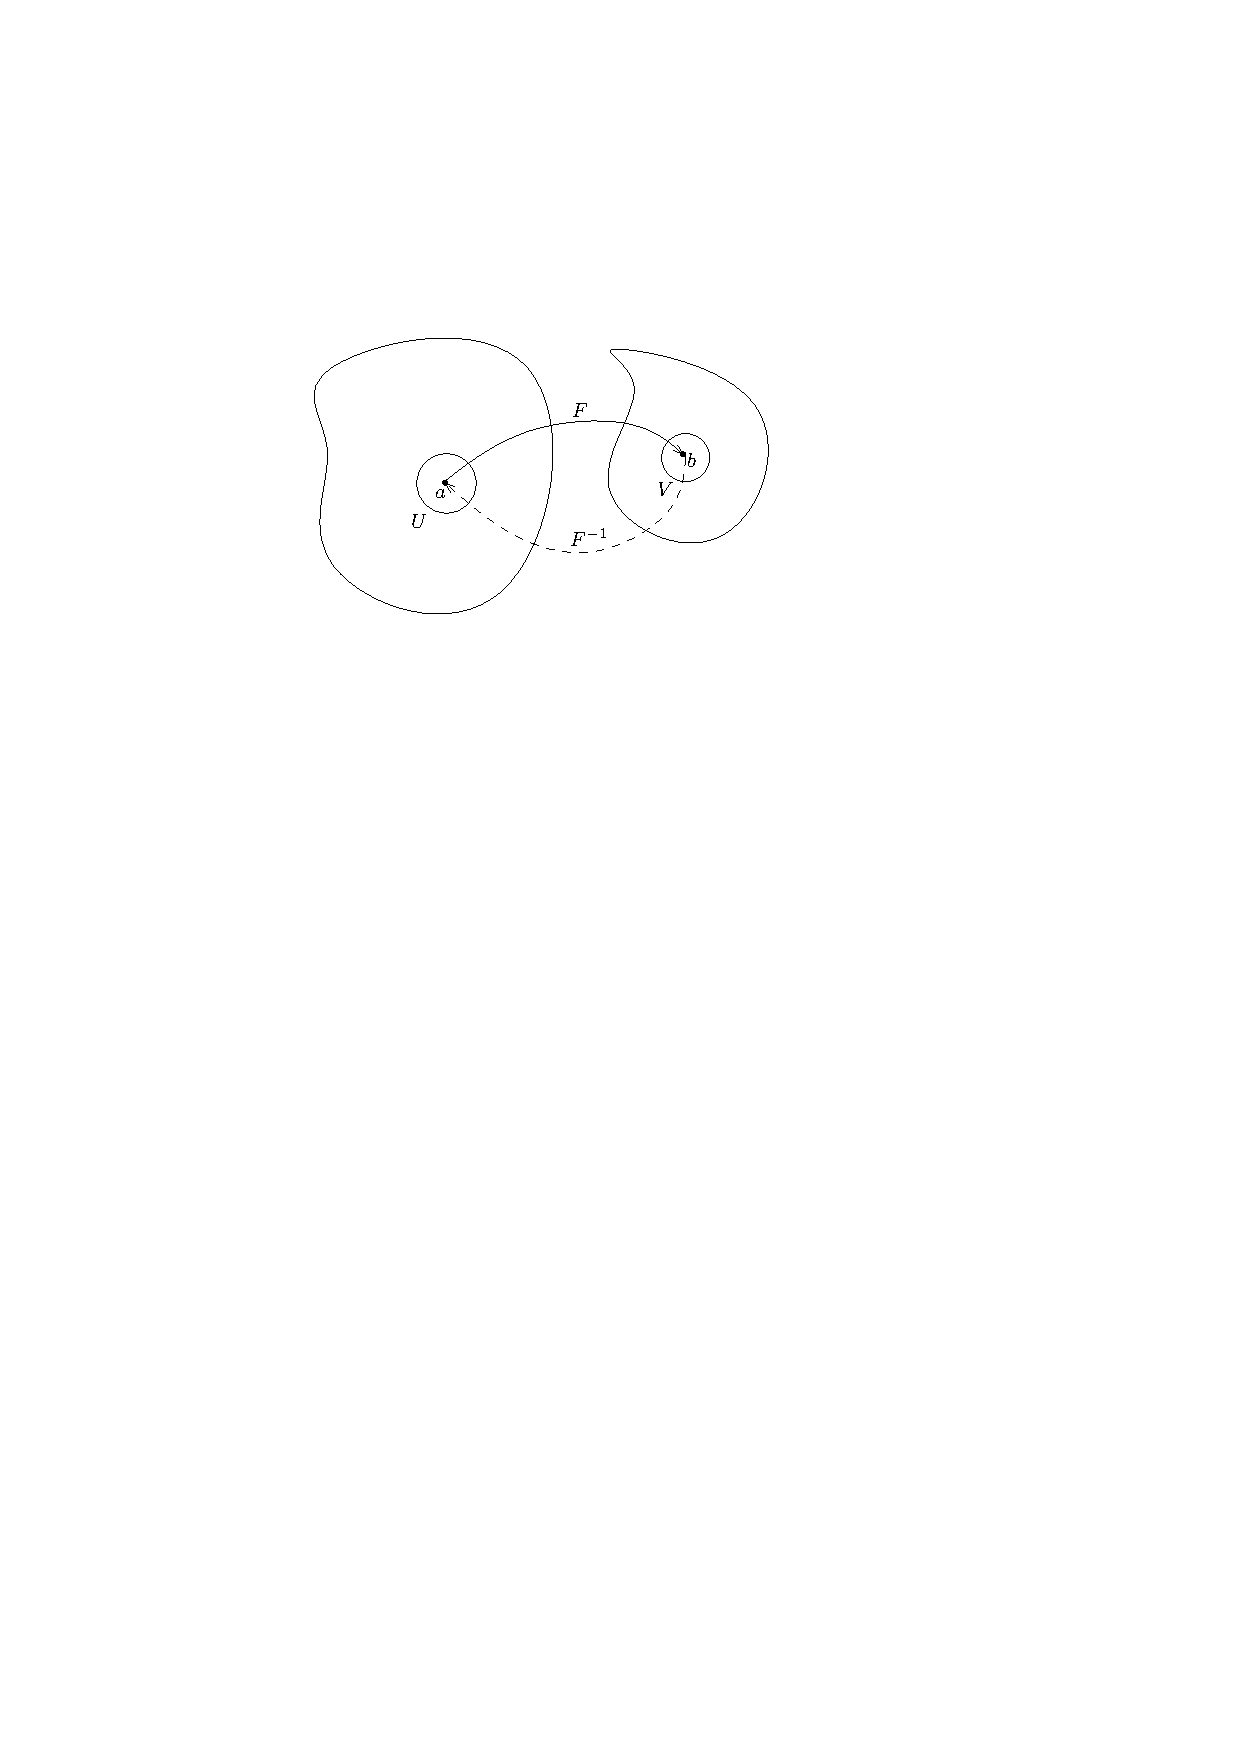
\includegraphics[width=0.6\linewidth]{inversemap}
\end{figure}

\begin{align}
  \Delta F &= F(x) - F(a) = y - b = \Delta y \label{eq:diffspace::invmaphandwave::delta}\\
  \Delta F &= F'(a) dx + o(dx) \\
  \del F(a) &= \del y(b) \label{eq:diffspace::invmaphandwave::diff}
\end{align}

Условие разрешимости \eqref{eq:diffspace::invmaphandwave::diff}~--- $\det\bigl(F'(a)\bigr) \neq 0$.
Утверждается, что \eqref{eq:diffspace::invmaphandwave::diff} $\Rightarrow$
\eqref{eq:diffspace::invmaphandwave::delta}

Соответственно, формулировка 
\begin{thrm}\label{thrm:diffspace::invmap}
  Пусть $F\colon G\subset \R^n \to \R^n$, $a\in G$, $b = F(a)$. Пусть ещё $F \in C^1$, 
  $\det(F'(a)) \neq 0$
  
  Тогда 
  \[
    \begin{split}
      & \exists\, U(a), V(b) \,\colon\; F \colon U \leftrightarrow V \\
      & \exists\, F^{-1} V\to U, \; F^{-1} \in C^1
    \end{split}
  \]
\end{thrm}

\paragraph{Доказательство теоремы об обратимости}
\label{par:diffspace::invmapproof}

\begin{ittproof}[Теорема об обратимости отображения]
  Введём обозначения:
  \begin{align*}
    F'(a) &= \Gamma\\
    \Phi(x) &= x - \Gamma^{-1} (F(x) - y)
  \end{align*}
  Нетрудно заметить, что $x$~--- неподвижная точка $\Phi$ (что $\Leftrightarrow F(x)=y$ ).
  Очень хотелось бы подогнать всё под теорему Банаха (\ref{thrm:diffspace::contrmap::banach}).
  Тогда отображение в окрестности $a$ будет взаимно-однозначным.

  \begin{enumerate}
    \item Сначала оценим $\|\Phi'\|$.
      \[
        \Phi'(x) = E - \Gamma^{-1} (F'(x)) = \Gamma^{-1} (F'(a) - F'(x))
      \]
      Можно норму оценить
      \[
        \|\Phi'(x)\| = \| \Gamma^{-1} \| \cdot \| (F'(a) - F'(x)) \|
      \]
      Последний множитель явно $\xrightarrow[x\to a]{} 0$ (так как $F\in C^1$)
      Тогда и $\|\Phi'(x)\|\to 0$. А значит найдётся $U_\varepsilon(a) \colon 
      \|\Phi'(x)\| \leqslant \frac{1}{2}$.
      
      Тогда по теореме \ref{thrm:diffspace::diffestim::diffestim} 
      \[
        x, x' \in U_\varepsilon(a) \Rightarrow \| \Phi(x) - \Phi(a)\| \leqslant \frac{1}{2}
        \|x-x'\|
      \]
      Собственно, почти победа. Осталось лишь выбрать внутри $U_\varepsilon$ компакт
      $\overline{U_{\varepsilon_1}}$ (иначе множество не очень полное).

    \item Теперь покажем, что 
      \[
        \exists\, \overline{U} \colon \Phi(U) \subset U  
      \]
      Попутно примем $\|y-b\| < \delta$, это потом поможет доказать непрерывность.
      \[
        \begin{split}
          \|\Phi(x) - a\| = \| x - a - \Gamma^{-1}(F(x)-y)\| 
          \leqslant \|\Gamma^{-1}\| \cdot \| \Gamma (x-a) - F(x) + y + b - b\| \\ 
          \leqslant \|\Gamma^{-1}\| 
          \cdot \bigl(\| - \underbrace{( F(x) - F'(a)(x-a) - F(a) )}_{\alpha}\| + \| y - b\| \bigr)
        \end{split}
      \]
      Выберем произвольный $\varepsilon \colon 0 < \varepsilon < \varepsilon_1$.
      
      Однако мы ещё можем подкрутить $\varepsilon_1$. 
      \[
        \exists\, U_{\varepsilon_1} \colon \frac{\|\alpha\|}{\|x-a\|} < \frac{1}{2\|\Gamma^{-1}\|}
      \]
      Это следует из формулы Тейлора (\ref{thrm:diffspace::taylor}), а применять её можно, так
      как шар~--- выпуклое множество. Ещё выберем $\delta = \frac{\varepsilon}{2\|\Gamma^{-1}\|}$.
      Там правда $\varepsilon$, а не $\varepsilon_1$.

      Тогда цепочка неравенств выше преобразуется к такому виду
      \[
        \ldots < \|\Gamma^{-1}\| \cdot \frac{\|x - a\|}{2\|\Gamma^{-1}\|} +
        \frac{\varepsilon}{2\|\Gamma^{-1}\|} \cdot \|\Gamma^{-1}\|
      \]

      А теперь положим $\|x-a\| \leqslant \varepsilon$ (неравенство нужно нестрогое для полноты). 
      Тогда
      \[
        x\in \overline{U_\varepsilon}(a) \Rightarrow \Phi(x) \in U_{\varepsilon}(a) \subset 
        \overline{U_\varepsilon}(a) 
      \]

      А теперь по теореме Банаха
      \[
        \exists!\, x_0\in \overline{U_\varepsilon}(a) \colon \Phi(x_0) = x_0 \Leftrightarrow
        F(x_0)= y_0 
      \]
      Видимо, осталось пересечь окрестность $a$ с прообразом $V(b)$ : $U = F^{-1}(V) \cap
      U_\varepsilon (a)$
      \item
      Заодно получилась и непрерывность:
      \[
        \forall\, U\; \exists\, V_\delta(b) \colon F^{-1}(V_\delta) \subset
        U_\varepsilon 
      \]
  \end{enumerate}
\end{ittproof}

\paragraph{Теорема о дифференцируемости обратного отображения}
\label{par:diffspace::invdiff}

\begin{thrm}[о дифференцируемости $F^{-1}$]\label{thrm:diffspace::invdiff}
  Пусть $U \subset \R^n$, $V \subset \R^n$, $F\colon U \leftrightarrow V$. Пусть также
  $F$~--- дифференцируемо в $a\in U$, $F(a) = b$,  $\det F'(a) \neq 0$. 
  Тогда $F^{-1}$ дифференцируемо в $b$.
\end{thrm}
\begin{ittproof}
  То, что есть обратное отображение, доказали выше. Пусть $y=F(x)$. Обозначим: $h= x-a$, $k=y-b$.
  Отображение биективно, значит $h\neq 0 \Leftrightarrow k \neq 0$.
  Из дифференцирумости $F$
  \[
    k = y - b = F(x) - F(a) = A h + \alpha \\
    \alpha = o(h) \; (h\to 0)
  \]
  $A = F'(a) \neq 0$, следовательно $\exists\, A^{-1}$
  \[
    A^{-1} k = A^{-1}Ah + A^{-1}\alpha \Rightarrow \Delta F^{-1} = h = A^{-1} k - A^{-1} \alpha
  \]
  Докажем, что $-A^{-1} \alpha =: \beta = o(k) \; (k\to 0) $
  \[
    \beta \leqslant \frac{-\alpha}{\|k\|} = \frac{-\alpha}{\|h\|}\cdot \frac{\|h\|}{\|k\|}  
  \]
  Покажем, что последнй член~--- ограничен
  \[
    \frac{\|h\|}{\|k\|} = \frac{\|h\|}{\|A h + \alpha\|} 
    \leqslant \frac{\|h\|}{\big|\|Ah\|- \|\alpha\|\big|}
    = \frac{1}{\big|\frac{\|Ah\|}{\|h\|} - \frac{\|\alpha\|}{\|h\|}\big|}  
  \]
  А последнее выражение ограничено при $\|h\| < \delta$

\end{ittproof}

\begin{cor*}
  $\displaystyle (F^{-1})'(b) = \bigl(F'(a)\bigr)^{-1}$
\end{cor*}

\paragraph{Теорема о гладкости обратного отображения}
\label{par:diffspace::invsmooth}

\begin{thrm}\label{thrm:diffspace::invsmooth}
  Пусть $F\colon U \leftrightarrow V$, биективна, $\in C^p$. Пусть к тому же $\det F'(x) \neq 0$.
  Тогда $F^{-1} \in C^p$
\end{thrm}
\begin{ittproof}
  Введём обозначения (оно всё существует по предыдущим теоремам хоть где-то)
  \[
    \begin{aligned}
      F'(x) &= \left(\frac{\partial F_i}{\partial x_j}\right)_{i,j=1}^n & &= (a_{ij}) = A \\
      (F^{-1})'(y) &= \left(\frac{\partial F^{-1}_i}{\partial y_j}\right)_{i,j=1}^n & &= (b_{ij}) = B 
    \end{aligned}
  \]
  Вполне ясно, что $B = A^{-1}$. Из алгебры $b_{ij} = \dfrac{\mathcal A_{ji}}{\det A}$ 
  (здесь $\mathcal A$~--- алгебраическое дополнение).
  
  Заметим, что из последнего выражения следует, что $b_{ij}$~--- рациональная функция от $\{a_{lk}\}$.
  Следовательно, $\widetilde{b_{ij}} = b_{ij}(a_{11}, \dotsc, a_{kl}, \dotsc, a_{nn}) \in C^\infty$.
  С другой стороны
  \[
    b_{ij}(y) = \frac{\partial F^{-1}}{\partial y_j}(y) = \frac{\partial F^{-1}}{\partial y_j}\bigl(F(x)\bigr)
    \Leftrightarrow b_{ij}(y) = \widehat{b_{ij}}(x)
  \]

  Так что $\widehat{b_{ij}} = b_{ij} \circ F$. 

  Дальше немного магии. Введём ещё одну функцию
  \[
    \overline{b_{ij}}(x) = b_{ij}(a_{11}(x), \dotsc, a{kl}(x), \dotsc, a_{nn}(x))   
  \]
  Заметим, что каждая $a_{ij}(x) \in C^{p-1} \Rightarrow \overline{b_{ij}} \in C^{p-1}$.
  Хорошо, тогда 
  \[
    b_{ij}(y) = \bigl(\overline{b_{ij}} \circ F^{(-1)}\bigr)(y) 
  \]
  Раньше доказали, что $F^{-1} \in C^0$. Теперь разматываем цепочку дальше:
  \[
    F^{-1} \in C^i \Rightarrow \overline{b_{ij}} \circ F^{-1} \in C^i \Rightarrow b_{ij} \in C^i 
  \]
  Значит, частные производные $F^{-1}$ принадлежат $C^i$. Тогда сама $F^{-1} \in C^{i+1}$.
  Таким бобром мы доберёмся до $C^p$. 
  Дальше не выйдет, так как не хватит гладкости $\overline{b_{ij}}$.
\end{ittproof}

\paragraph{Гладкая зависимость корней многочлена от его коэффициентов}
\label{par:diffspace::smoothpolyroots}

\begin{thrm}\label{thrm:diffspace::smoothpolyroots}
  Пусть $P(x) \in \R[x]$ имеет $n$ корней $(x^0_j)$,  $x^0_j \in \R$, таких что $\forall\, i,j \; x^0_i \neq x^0_j$.  
  Тогда 
  \[
    x_i = x_i(a_0, \dotsc, a_{n-1}) \in C^\infty
  \]
\end{thrm}

\begin{ittproof}
  Пусть $P(x) = (x - x_1) \dotsm (x - x_n)$. Вспомним теорему Виета (из алгебры)
  \begin{align*}
    a_0     & = (-1)^n x_1 \dotsm x_n \\
    a_1     & = (-1)^{n-1} \sum_{i} \prod_{j \neq i} x_j \\
            & \cdots \cdots \cdots  \\
    a_{n-1} & = (-1) \sum_i x_i
  \end{align*}

  Рассмотрим $P$ как отображение $(x_1, \dotsc, x_n) \mapsto (a_0, \dotsc, a_{n-1})$.
  \[
    P'(x) = 
    \begin{pmatrix}
      \frac{\partial P_1}{\partial x_1} & \cdots & \frac{\partial P_1}{\partial x_n} \\
      \vdots & \ddots & \vdots \\
      \frac{\partial P_n}{\partial x_1} & \cdots & \frac{\partial P_n}{\partial x_n} \\
    \end{pmatrix}
    = 
    \begin{pmatrix}
      (-1)^n \prod_{i\neq 1} x_i & (-1)^n \prod_{i\neq 2} x_i & \cdots & (-1)^n \prod_{i\neq n} x_i \\
      \hdotsfor{4} \\
      -1 & -1 & \cdots & -1 
    \end{pmatrix}
  \]
  Посчитаем $\det(F')$. Этот определитель можно рассмотреть как многочлен $\in R[x_1, \dotsc, x_n]$
  Его степень не превосходит $0 + 1 + \dotsb + (n-1) = \frac{n(n-1)}{2}$. Заметим, что если хоть
  какая-то пара столбиков равны, то определитель равен нулю. Так что $\det(F')$ делится на
  всевозможные многочлены вида $x_i - x_j$. А их как раз $\frac{n(n-1)}{2}$ и они неприводимые.
  Следовательно, 
  \[
    \det (F')(x_1, \dotsc, x_n) = C \prod_{i<j} (x_i - x_j) 
  \]
  А значит при условии неравенства корней он ненулевой.
  \footnote{Этого, конечно, не было в курсе алгебры, но там не используется ничего страшнее
  теоремы о делении с остатком. Вообще доказать бы надо, но лень.}

  Дальше можно воспользоваться теоремой о гладкости обратного отображения.
\end{ittproof}

\paragraph{Теорема о неявном отображении}
\label{par:diffspace::implicit}

\verb+20:07 2016-10-15+

\begin{defn}\label{defn:diffspace::implicit}
  Пусть $F \colon \R^m\times\R^n \to \R^m$. Рассмотрим уравнение
  \begin{equation}
    F(x, y) = 0
    \label{eq:diffspace::impicit::baseeq}
  \end{equation}
  Пусть $x^0\in \R^n$, $y^0\in \R^k$ такие, что $F(x^0, y^0) = 0$.
 
  Тогда если $\exists\,P(x^0) \subset \R^n$, $Q(y^0) \subset \R^m$, такие что
  \[
    \forall\, x\in P \; \exists!\, y\in Q \colon F(x,y) = 0
  \]
  то говорят, что уравнение \eqref{eq:diffspace::impicit::baseeq} задаёт неявную функцию 
  $f\colon P \to Q$.
\end{defn}

Сначала всякие комментарии.
\begin{equation*}
  \text{\eqref{eq:diffspace::impicit::baseeq}} \Leftrightarrow
  \begin{cases}
    F_1(x_1, \dotsc, x_n, y_1, \dotsc, y_m) = 0 \\
    \hdotsfor{1}\\
    F_k(x_1, \dotsc, x_n, y_1, \dotsc, y_m) = 0 \\
  \end{cases}
\end{equation*}

Как обычно, главная идея состоит в том, чтобы всё линеаризовать
\begin{equation}
  \begin{cases}
    \del F_1 = 0 \\
    \hdotsfor{1}\\
    \del F_k = 0 \\
  \end{cases}
  \Leftrightarrow 
  \begin{cases}
    \sum_{j=1}^m \frac{\partial F_1}{\partial y_j}\, \del y_j = 
    \sum_{j=1}^m \frac{\partial F_1}{\partial x_j}\, \del x_j \\
    \hdotsfor{1}\\
    \sum_{j=1}^m \frac{\partial F_k}{\partial y_j}\, \del y_j = 
    \sum_{j=1}^m \frac{\partial F_k}{\partial x_j}\, \del x_j .\\
  \end{cases}\nolinebreak\label{eq:diffspace::impicit::diff}
\end{equation}
При этом $\del y_j$ мы хотим выразить через $\del x_j$.
Какие-то шансы обратить всё это дело есть лишь при условиях:
\begin{enumerate}
  \item $k=m$
  \item $\det \left(\dfrac{\partial(F_1, \dotsc, F_k)}{\partial(y_1, \dotsc, y_m)}\right) \neq 0$
\end{enumerate}

Сейчас будем доказывать, что \eqref{eq:diffspace::impicit::diff} $\Rightarrow$ \eqref{eq:diffspace::impicit::baseeq}.


\begin{thrm}[Теорема о неявном отображении]\label{thrm:diffspace::implicit}
  Пусть $F\colon G \subset \R^n \times \R^m \to \R^m $, $F \in C^p$, $p \geqslant 1$.
  \[
    F(x, y) = 0, \;\; (x_0, y_0) \in G
  \]
  \begin{enumerate}
    \item $F(x_0, y_0) = 0 $
    \item $\det F_y'(x_0, y_0) \neq 0$
  \end{enumerate}

  Тогда $\exists\, P(x_0), Q(x_0)$, такие, что \eqref{eq:diffspace::impicit::baseeq} задаёт
  неявное отображение $f\colon P \to Q$. При этом $f\in C^p$ и 
  \[
    f'(x) = - \bigl(F_y'(x,y)\bigr)^{-1} \cdot F_x'(x,y)
  \]
\end{thrm}

\begin{ittproof}
  Доказательство~--- <<обёртка>> над теоремой об обратном отображении. 
  К слову, в \cite[c.~673]{zorich1} сразу доказывается утверждение о неявном отображении.

  Итак, обозначения:
  \begin{enumerate}
    \item $\Phi\colon G \subset \R^n\times\R^m \to \R^n\times\R^m$. Работает как-то так:
      \[
        (x, y) \mapsto (u, v) , \;
        \begin{dcases}
          u = x, & u \in R^n \\
          v = F(x,y) , & v\in \R^m
        \end{dcases}
      \]
    \item $i\colon \R^n \to \R^n \times \R^m$ такого сорта $x \mapsto (x, 0)$
    \item $\pi \colon \R^n \times \R^m \to \R^m$ такого сорта $(x,y) \mapsto y$
  \end{enumerate}

  Теперь найдём определитель $\Phi'(x,y)$. Посчитав как-то частные производные, получим
  \[
    \Phi'(x,y) = 
    \left(
      \begin{array}{c|c}
        E_n    & 0 \\
        \hline
        F_x'   &  F_y'
      \end{array}
    \right) \Rightarrow \det \bigl(\Phi'(x_0,y_0) \bigr) = \det E_n \cdot \det F_y'(x_0, y_0) \neq 0
  \]
  Чудно, значит по теореме об обратном отображении (\ref{thrm:diffspace::invmap}) 
  $\exists\, \Phi^{-1}(x_0, y_0)$ и ещё окрестности $U(x_0, y_0), V(x_0, 0)$.
  Теперь определим окрестности из условия теоремы:
  \[
    P(x_0) = i^{-1}(V) \; \land \; Q(y_0) = \pi(U)
  \]
  По сути~--- проекции.
  
  В таких обозначениях $f = \pi \circ \Phi^{-1} \circ i$. Вполне очевидно, что $f \in C^p$.
  Ну $i, \pi \in C^\infty, \; \Phi^{-1} \in C^p$. 

  К тому же
  \[
    \forall\, x \in P \; x \overset{i}{\mapsto} (x, 0) \overset{\Phi^{-1}}{\mapsto} (x,y) 
    \overset{\pi}{\mapsto} y \in Q 
  \]
  При этом такой $y$~--- единственный. В итоге получилось задать неявно отображение $f$.

  Из вышесказанного, оно сколько нужно раз дифференцируемо. Так что
  \[
    \pder{}{x} F(x, f(x)) = F_x' \cdot E + F_y' \cdot f'(x) = 0
  \]
  По условию $F_y'$~--- обратима. Следовательно,
  \[
    f'(x) = - (F_y'(x,y))^{-1} \cdot F_x'(x,y)
  \]
  
\end{ittproof}

\paragraph{Функциональная зависимость системы функций}
\label{par:diffspace::funcdep}

\begin{defn}\label{defn:diffspace::funcdep}
  Пусть $f_1, \dotsc, f_m, g \colon G \subset \R^n \to \R$~--- гладкие функции, $x_0 \in G$.
  Тогда эти функции называются функционально зависимыми в $V(x_0)$, если
  \[
    \exists\, \varphi\colon U(f(x_0)) \to \R, \varphi \in C^1 \; \colon \; g(x) = \varphi(f(x)) 
    \text{ в } V(x_0)  
  \]
\end{defn}
\begin{defn}\label{defn:diffspace::funcindep}
  Пусть $f_1, \dotsc, f_m, g \colon G \subset \R^n \to \R$~--- гладкие функции. Тогда эти функции
  называются функционально \emph{не}зависимыми, если определение выше не выполняется ни для какой
  $V \subset G$
\end{defn}
\begin{rem*}
  Тут лажа какая-то c определениями, не отрицание же нифига.
\end{rem*}

\verb+ 2016-10-16 13:21 +

\begin{thrm}(о функциональной зависимости)\label{thrm:diffspace::funcdep}
  Пусть $f_1, \dotsc, f_m, g \colon G \subset \R^n \to \R$~--- гладкие функции. К тому же
  $a\in G$, $f = (f_i)_i$, $y = f(x)$, 
  $
    \rk \begin{pmatrix}
      f_1' \\ \vdots \\ f_m' 
    \end{pmatrix} = m
  $ в точке $x\in U(a)$.
  Тогда, если 
  $
    \rk \begin{pmatrix}
      f_1' \\ \vdots \\ f_m' \\ g' 
    \end{pmatrix} = m
  $ в точке $x \in U(a)$, то $\exists\, V(a)$ в которой $g$ функционально зависит от $f_1, \dotsc,
  f_m$.
\end{thrm}
\begin{ittproof}
  Пусть сразу $n \geqslant m$, иначе условие теоремы не выполняется совсем никогда (ну там m
  векторов всегда ЛЗ).

  Введём обозначения:
  \[
    x = (\underbrace{x, \dotsc, x_m}_{\bar{x}}, \underbrace{x_{m+1}, \dotsc,
    x_n}_{\bar{\bar{x}}}), \; \bar y = (y_1, \dotsc, y_m, \bar{\bar x})
  \]

  Из алгебры в $f'(x), x\in U(a)$ существует ненулевой минор порядка $m$. Можно НУО считать, что он
  соответствует $\bar x$. Тогда это равносильно тому, что $\displaystyle \det \left(\pder{f}{\bar
  x}(a)\right) \neq 0$.

  Рассмотрим такую неявную функцию 
  \[
    F \colon \R^n \times \R^m \to \R^m, \; F(\bar{y}, \bar{x}) = y - f(\bar{x}, \bar{\bar x}) = 0 
  \]
  Оно всё по условию гладкое.
  Тогда по теореме о неявном отображении существует пара окрестностей $P, Q$ и 
  \[
    \exists\,\varphi \colon P\subset \R^n \to Q\subset \R^m, \;  \bar x = \varphi(\bar y)
  \] 
  В этих окрестностях $F\equiv 0 \Leftrightarrow y \equiv f(\varphi(y, \bar{\bar x}), \bar{\bar x})$.
  Заметим, что здесь $y, \bar{\bar x}$~--- независисые переменные. Так что если $j > m$, то
  \[
    \pder{}{x_j} f_i(\varphi(\bar y), \bar{\bar x}) = \sum_{k=1}^m \partial_k{f_i} \cdot
    \pder{\varphi_k}{x_j} + \partial_j f_i \equiv 0
  \]

  Из условия на ранг известно, что 
  \[
    g'(x) = \sum_{i=1}^m \lambda_i f_i'(x), \; x\in U(a)
  \]

  Нам для того чтобы показать, что $g$ функционально зависит от $f$, необходимо приравнять в
  окрестности точки $a$ $g$ к функции от $y$. Пусть снова $j>m$, тогда 
  \begin{align*}
    & g(x) = g(\bar x, \bar{\bar x}) = g(\varphi(\bar y), \bar{\bar x}) \\
    &\pder{g}{x_j}  = \sum_{k=1}^m \partial_k g \cdot \pder{\varphi_k}{x_j} + \partial_j g 
  \end{align*}
  А вот теперь нужно воспользоваться условием на ранги. Тут очень важно, что это условие работает
  в окрестности $a$~--- ведь какие-то тождества в точке нам ничего интересного не дадут.
  \[
    \pder{g}{x_j}  = \sum_{i=1}^m \lambda_i \left(\partial_k f 
    \cdot \pder{\varphi_k}{x_j} + \partial_j f_i\right) = 0 
  \]
  Из того, что $g, \varphi$~--- гладкие получаем, что и функция, нужная в определении
  \ref{defn:diffspace::funcdep} тоже гладкая. Вроде всё.
\end{ittproof}




\end{document}
% vim: wrapmargin=3

\chapter{Криволинейные интегралы}
%------------------------------------------------------------
% Description : Line integrals, diff forms
% Author      : taxus-d <iliya.t@mail.ru>
% Created at  : Sun Nov 13 16:01:51 MSK 2016
%------------------------------------------------------------
\documentclass[12pt,timbord]{../../../notes}
\usepackage{silence}
\WarningFilter{latex}{Reference}
\graphicspath{{../../img/}}

\begin{document}
\paragraph{\underdev Интеграл от дифференциальной формы по пути}
\label{par:lineint::defs}
Параграфы со значком  <<\underdev>> лучше не читать, они недопилены.

\subparagraph{Дифференциальные формы.} 
Начать лучше с полилинейных форм.
\begin{defn}\label{defn:lineint::defs::linform}
  Пусть $L$~--- линейное пространство над полем $K$. Тогда функция $A\colon L^k\to K$, линейная по
  каждому из своих аргументов, называется $k$-линейной формой.
\end{defn}

\note{<ну его>}\note{<потом лучше напишу>}

Нам тут хватит и 1-форм, так что
\begin{defn}\label{defn:lineint::defs::diffform}
  Дифференциальной 1-формой можно назвать отображение из $\R^n$ в линейную (по $h$) форму, $P\in C^0$
  \[
    \omega = \langle P(x), \del x(x,h)\rangle
  \]
  Но это как-то не очень ({а что такое дифференциал?}).
\end{defn}

\subparagraph{Гладкие пути.}

\begin{defn}\label{defn:lineint::defs::smoothpath}
  Пусть $\gamma\colon [a;b]\subset \R \to \R^n$. Тогда $\gamma$ называется путём в пространстве
  $\R^n$.
  \begin{itemize}
    \item Путь гладкий, если $\gamma\in C^1$,
    \item путь регулярный, если $\rk\gamma' \geqslant 1$,
    \item путь простой, если $\gamma$~--- биекция.
  \end{itemize}
\end{defn}

\begin{defn}\label{defn:lineint::defs::curve}
  Образ $\Gamma = \gamma([a;b]) \subset \R^n$ называется \emph{кривой} в $\R^n$. Ещё говорят, что
  $\Gamma$~--- носитель пути $\gamma$, а $\gamma$~--- параметризация $\Gamma$. \note{здесь ещё
  можно как в \cite{shabat} определять кривую как класс эквивалентности путей, так вроде проще}
\end{defn}

\begin{rem*}
  Путь простой $\Leftrightarrow$ кривая не имеет самопересечений.
\end{rem*}

\begin{defn}\label{defn:lineint::defs::pathorient}
  Будем говорить, что простые пути имеют одинаковую ориентацию, если
  \[
    \gamma_1(a_1)=\gamma_2(a_2)\; \gamma_1(b_1) = \gamma_2(b_2)
  \]
  и противоположную, если всё наоборот.
  Тут ещё введу нестандартное обозначение, но так жить проще $\ddot\smile$.
  \begin{itemize}
    \item $\coori$~--- одинаковая ориентация
    \item $\conori$~--- противоположная ориентация
  \end{itemize}
\end{defn}
\begin{rem*}
  Для биективных параметризаций видимо просто нет другого выбора. С петлями всё будет интереснее.
\end{rem*}

\subparagraph{Интегралы от форм по пути}

\begin{defn}\label{defn:lineint::defs::lineint}
  Просто возьмём и определим интегралы по простому гладкому пути от 1-форм так:
  \[
    I = \int_\gamma \omega := \int_a^b \langle P,\dot x(t)\rangle \del t
  \]
\end{defn}

\begin{prop}[Корректность определения выше]\label{prop:lineint::defs::lineint}
  Интеграл по пути не зависит от параметризации.
\end{prop}
\begin{ittproof}
  Пусть $\gamma_1, \gamma_2$~--- параметризации $\Gamma$, одинаково ориентированы. Докажем,что
  \[
    I_1 = \int_{\gamma_1} \omega = \int_{\gamma_2} \omega = I_2 
  \]
  Поскольку $\gamma_1, \gamma_2$~--- биекции, $\exists\, \varphi \colon $
  $t_2 = \varphi(t_1)$, тоже биекция, такого сорта:
   $t_1\xmapsto{\gamma_1}x\xmapsto{\gamma_2^{-1}}t_2$
  Тогда 
  \[
    I_2  = \int_{a_2}^{b_2} \langle P(\gamma_2(t_2)), \partial_{t_2}\gamma_2(t_2)\rangle \,\del t_2 = 
    \int_{a_1}^{b_1} \langle P(\underbrace{\gamma_2(\varphi(t_1))}_x), 
  \partial_{t_2}\gamma_2(t_2))\rangle \, \partial_{t_1}\varphi(t_1) \,\del t_1
  \]
  Покажем, что $\partial_{t_2}\gamma_2(t_2) \partial_{t_1}\varphi = \partial_{t_1}
  \gamma_1(t_1)$. Это просто следует равенства $\gamma_1(t_1)=\gamma_2(t_2)$, если его
  продифференцировать по $t_1$. Так что
  \[
    \int_{a_1}^{b_1} \langle P(x), 
  \partial_{t_1}\gamma_1(t_1))\rangle \, \bigl(\partial_{t_1}\varphi(t_1) \bigr)^{-1}
  \partial_{t_1}\varphi(t_1) \,\del t_1   = I_1
  \]
\end{ittproof}
\begin{rem}
  Если $\gamma_1 \conori \gamma_2$, то $I_2 = - I_1$.
\end{rem}
\begin{rem}
  Если рассматривать только одинаково ориентированые пути, то
  \[
    \int_{\gamma} \omega = \int_{\Gamma} \omega
  \]
\end{rem}

\begin{rem}
  Если $\Gamma$ разбивается на непересекащиеся $\Gamma_1$, $\Gamma_2$, то 
  \[
    \int_\Gamma \omega = \int_{\Gamma_1} \omega + \int_{\Gamma_2} \omega
  \]
\end{rem}

\subparagraph{Петли и интегралы по ним}


\begin{defn}\label{defn:lineint::defs::loop}
  Кривая $\Gamma$~--- петля, если для всякой её параметризации $\gamma(a) = \gamma(b)$. 
  Петля называется простой, если $\exists\, \colon \gamma\vert_{[a;b)}$~--- биекция.
\end{defn}
\begin{rem*}
  Плохие петли можно разбивать на простые.
\end{rem*}

\begin{defn}\label{defn:lineint::defs::loopint}
  Пусть $\Gamma$~--- простая петля. Тогда 
  \[
    I = \oint_\gamma \omega := \int_a^b \langle P,\dot x(t)\rangle \del t
  \]
\end{defn}
\begin{prop}\label{prop:lineint::defs::loopint}
  Определение выше корректно, и не зависит от выбора <<начала>> петли. 
\end{prop}  
\begin{itlproof}
  Можно рассмотреть 2 разные параметризации и разбить на 2 куска. Дальше работает определение
  интеграла по простому пути.
\end{itlproof}

\begin{rem*}
  Чтобы посчитать интегралы по всем остальным путям, их нужно разбивать на прострые пути и
  простые петли
\end{rem*}


\paragraph{Точные формы}
\label{par:lineint::precforms}

\begin{defn}\label{defn:lineint::precforms::def}
  1-форма $\omega$ называется точной в $G$, если $\exists\, \Phi\colon G\subset \R^n\to \R$, такая что
  $\omega =  \del \Phi$. $\Phi$ в таком случае называется потенциалом, а сама форма ещё иногда
  назыается потенциальной.
\end{defn}
\begin{exmp*}
  Работа в физике.
\end{exmp*}

\begin{thrm}\label{thrm:lineint::precforms::precint}
  Пусть $\omega$~--- точная форма в  $G$, $\Gamma \subset G$, $\gamma(a)=A$, $\gamma(b)=B$
  Тогда
  \[
    \int_\gamma \omega = \Phi(B) - \Phi(A)
  \]
\end{thrm}
\begin{ittproof}
  $\langle P, x \rangle = (\Phi \circ \gamma)' (t)$. Дальше уже тривиально из непрерывности
  $\Phi$.
\end{ittproof}

\begin{thrm}\label{thrm:lineint::precforms::precint2}
  Пусть $\omega$~--- точная форма в  $G$, $\Gamma_1, \Gamma_2 \subset G$,
  $\gamma_{1,2}(a)=A$, $\gamma_{1|2}(b)=B$.
  Тогда
  \[
    \int_\gamma \omega = \Phi(B) - \Phi(A)
  \]
\end{thrm}

\begin{thrm}\label{thrm:lineint::precforms::loopint}
  Пусть $\omega$~--- точная форма в  $G$, $\Gamma \subset G$~--- петля
  Тогда
  \[
    \oint_\gamma \omega = 0
  \]
\end{thrm}

\begin{thrm}\label{thrm:lineint::precforms::critprec}
  Пусть $\omega$~--- форма в  $G$, и $\int_\gamma \omega $ не зависит от пути при фиксировнных
  концах. Тогда $\omega$~--- точна.
\end{thrm}

\begin{ittproof}
  Надо показать, что $\partial_i \Phi = P^i$. В этом месте можно забить на общности и объявить
  $n=2$. Докажем, что $\partial_x \Phi = P^1$. Поскольку от пути ничего не зависит,
  \[
    \pder{\Phi}{x}(x,y) = \lim_{\Delta x\to 0}\frac{\Phi(x+\Delta x)- \Phi(x,y)}{\Delta x} = 
    \lim_{\Delta x\to 0} \frac{1}{\Delta x} \left(\int_A^{{(x+\Delta x,y)}} \omega - 
    \int_A^{(x,y)} \omega\right)
  \]
  А это по сути интеграл по пути, соединяющем $(x+\Delta x, y)$ и $(x, y)$. А здесь уже можно
  взять приличную кривую (прямую) с правильной параметризацией, и воспользоваться теоремой о
  среднем.
  \[
    \cdots = \lim_{\Delta x \to 0} \frac{1}{\Delta x} \int_{x}^{x+\Delta x} P(t, y) \del t = 
    \lim_{\Delta x \to 0} P(\xi, y) = P(x,y)
  \]
  Последнее равенство верно по непрерывности.
\end{ittproof}

\begin{thrm}\label{thrm:lineint::precforms::critprecloop}
  $\displaystyle \oint \omega =0 \Rightarrow \omega$~--- точна
\end{thrm}

\begin{thrm}\label{thrm:lineint::precforms::precrecloop}
  Пусть $G$, $\oint \omega =0 $ для любой прямоугольной петли. Тогда $\omega$~--- точна.
\end{thrm}
\begin{ittproof}
  Аккуратно свести к теореме~\ref{thrm:lineint::precforms::critprec}, там всё будет работать и с
  путями, параллельными осям координат.
\end{ittproof}

\paragraph{Замкнутые формы}
\label{par:lineint::closforms}
Здесь уже окончательно забиваем на все $n \geqslant 2$. Там, в целом, понятно как обобщать.
Тут всюду $\omega =  P(x,y) \del x + Q(x,y) \del y$
\begin{defn}\label{defn:lineint::closforms::closform}
  Форма $\omega$ замкнута в $G$, если
  \[
    \forall\, A \in G \; \exists U (A) \colon \exists\, \Phi_U\colon U\to R \;\:\: \omega = \del
    \Phi_U
  \]
  короче, локально точна.
\end{defn}

\begin{thrm}\label{thrm:lineint::closforms::nessdiff}
  Пусть $\omega$~--- гладкая форма в $G$. Тогда если $\omega$ замкнута,
  $\partial_y P = \partial_x Q$ в $G$.
\end{thrm}
\begin{ittproof}
  Очевидно следует из <<локальной точности>>.
\end{ittproof}

\begin{thrm}\label{thrm:lineint::closforms::suffdiff}
  Пусть $\omega$~--- гладкая форма в $G$. Тогда если $\partial_y P = \partial_x Q$ в $G$, то
  $\omega$ замкнута.  
\end{thrm}
\begin{ittproof}
  Выберем произвольную $A$, тогда $U_\varepsilon(A) \subset G$. Надо попробовать построить
  потенциал. Например так $\Phi(B) = \int_{\gamma_1 + \gamma_2} \omega$. 
  Докажем, что $\partial_x \Phi = P$, $\partial_y \Phi = Q$.

  \begin{minipage}{0.48\linewidth}
    \begin{tikzpicture}[scale=2]
      \coordinate[label=$A$] (A) at (0,0);
      \coordinate[label=$B$] (B) at (0.7,1);
      \coordinate[label=$C$] (C) at (1.1,1);
      \coordinate (D) at (0.7,0);
      \coordinate (E) at (1.1,0);
      \draw (0,0) circle (2);
      \begin{scope}[decoration={
            markings,
          mark=at position 0.5 with {\arrow{>}}}
        ] 
        \draw[postaction={decorate}] (A)-- node[below]{$\gamma_1$} (D);
        \draw[postaction={decorate}] (D)-- node[left]{$\gamma_2$}(B);
        \draw[postaction={decorate}] (D)-- node[below]{$\gamma_3$}(E);
        \draw[postaction={decorate}] (E)-- node[right]{$\gamma_4$}(C);
      \end{scope}
    \end{tikzpicture}
  \end{minipage}\hfill
  \begin{minipage}{0.48\linewidth}
    \[
      \begin{split}
        \Delta \Phi &= \Phi(C)-\Phi(B) = \int_{\gamma_4} \omega - \int_{\gamma_2} \omega +
        \int_{\gamma_3} \omega \\
        &= \int_{y_A}^y Q(x+\Delta x, t) \del t 
        - \int_{y_A}^y Q(x, t) \del t + \int_{x}^{x+\Delta x} P(t, y_A) \del t
      \end{split}
    \]
    Последний сходится к $P(x,y_0)\del x$, а первые два надо немного преобразовать
    \[
      \frac{1}{\Delta x} \left(\int_{\gamma_4} \omega 0 \int_{\gamma_2} \omega \right)
      = \int_{y_0}^y \left(\frac{Q(x+\Delta x,t ) - Q(x,t)}{\Delta x}\right) \del t
    \]
    Подинтегральную функцию можно представить как последовательность $f_n \rightrightarrows Q'$.
    \[
      \left| \frac{Q(x+\lfrac 1 n )- Q(x)}{\frac 1 n} - Q'(x)\right| = |Q'(\xi) - Q(x) |
      <\varepsilon
    \]
    а функция $Q'$ равномерно непрерывна на $[x, x+ \Delta x]$, ибо он отрезок. Так что можно
    поменять местами предел и интеграл.
    \[
      \cdots = \int_{y_0}^y \pder{Q}{x}(x,y) \del t = \int_{y_0}^y \pder{P}{y} (x,y) = \Delta P
    \]
  \end{minipage}
    Если сложить с оставшимся куском, то как раз и выйдет $P$. С равенством $Q$ вроде все
    попроще, там нужно считать приращение всего лишь по одному пути.
\end{ittproof}
\begin{rem}
  Бывают замкнутые, но не точные формы. Например $\omega = \dfrac{-y \del x + x \del y}{x^2 +
  y^2}$. Она замкнута, а вот $\oint_\gamma w$ по окружности вокруг $0$ не 0.
\end{rem}

\paragraph{Первообразная замкнутой формы вдоль пути}
\label{par:lineint::closintpath}

Сначала можно отметить, что $\Gamma = \gamma\bigl([a;b]\bigr)$~--- компакт. Так что вроде можно
пользоваться теоремой о конечном подпокрытии.
\begin{lem}\label{thrm:lineint::closintpath::potdiff}
    Пусть $G$~--- область, $\omega$~--- гладкая точная форма в $G$, 
    а $\Phi, \Psi$~--- две её первообразные в $G$. Тогда $\Phi-\Psi\equiv C\in \R$.
\end{lem}

\begin{thrm}\label{thrm:lineint::closintpath}
  Пусть $\omega$ замкнута в $G$, $\Gamma=\gamma([a;b])$. Тогда существует первообразная вдоль пути
  $\gamma$ и  $\dint_\gamma \omega = f(b) - f(a)$.
\end{thrm}

\begin{ittproof}
  Поскольку кривая компактна, в любом её покрытии можно выделить конечное подпокрытие. Собственно,
  будем рассматривать покрытие открытыми кругами $U(p_i)$. Пусть $\Phi_i$~--- произвольная
  первообразная в $U_i$. Заменим $\Phi_i$ $\widetilde{\Phi_i}$, так что 
  $\widetilde{\Phi}_{i+1}= \widetilde{\Phi}_{i}$ на $U_{i+1} \cap U_i$, $\widetilde{U}_0=U_0$.

  Выберем параметризацию, тогда $p_i$  соответствуют $t_0=a< t_1 <\cdots < t_n = b$
  Теперь выберем $f(\gamma(t)) = \widetilde{\Phi}_k(\gamma(t))$, $\gamma(t) \in U_k$.
  Здесь вроде можно прожить и без простоты пути.\note{вообще первообразную вдоль пути нигде не
  определяли, так что можно считать конструкцию, построенную выше, определением}

  Теперь ещё выберем $q_i \in U_{i+1} \cap U_i$, $\{\gamma_j\} =$ пути от $ p_i$ до $q_i \cap$
  пути от $q_i$ до $p_{i+1}$. Тогда
  \[
    \in _\gamma \omega = \sum_j\int_{\gamma_j} =  \widetilde{\Phi}(p_n) - \widetilde{\Phi}{p_0} =
    f(b) - f(a)
  \]
\end{ittproof}

\paragraph{\underdev Гомотопия путей}
\label{par:lineint::homotopy}

\begin{defn}\label{defn:lineint::homotopy::set}
  Непрерывным семейством путей называется непрерывная функция $g\colon [0;1]\times[a;b]\to \R^n$.
  Часто обозначается так: $\gamma_s(t) = g(s,t)$. \note{По-хорошему там должны быть топологические
  пространства, но не сегодня и не сейчас .}
\end{defn}

\begin{defn}[$\ddot\sim$]\label{defn:lineint::homotopy::paths}
  Пусть $\gamma_1, \gamma_2\colon [a;b]\to G$, $\gamma_1(a)=
  \gamma_2(a)$,$\gamma_1(b)=\gamma_2(b)$. Тогда утверждается, что пути гомотопны, если существует
  семейство $\gamma_s(t)\colon$ $\gamma_{s_1} = \gamma_1$, $\gamma_{s_2} = \gamma_2$.
\end{defn}
\begin{rem*}
  Таки отношение эквивалентности.
\end{rem*}

\begin{thrm}\label{thrm:lineint::homotopy::lineinteq}
  Пусть $\omega$~--- замкнутая форма в области $G$, $\gamma_1 \sim \gamma_2$. Тогда
  \[
    \int _{\gamma_1} \omega = \int_{\gamma_2} \omega
  \]
\end{thrm} 
\begin{thrm}\label{thrm:lineint::homotopy::loopinteq}
  Пусть $\omega$~--- замкнутая форма в области $G$, $\gamma_1 \sim \gamma_2$~--- гомотопные петли.
  Тогда
  \[
    \oint _{\gamma_1} \omega = \oint_{\gamma_2} \omega
  \]
\end{thrm} 
\begin{rem*}
  Доказывать я это пока не буду, иначе это будет выглядеть как-то так:\par
  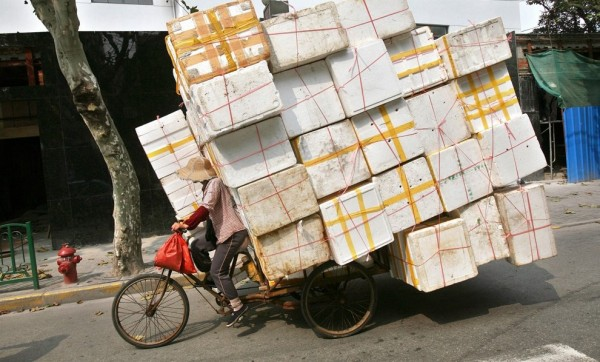
\includegraphics[width=0.7\linewidth]{overloaded}
\end{rem*}

\begin{cor}\label{imp:lineint::homotopy::loophomdot}
  Пусть $\gamma$~--- петля в $G$ и $\gamma \mathop{\overset{G}{\sim}} \bullet$. Тогда
  $\displaystyle\oint_\gamma w = 0$.
\end{cor}



\begin{defn}\label{defn:lineint::homotopy::simpconn}
  Область в $G$ называется односвязной, если в ней всякая петля стягивается в точку.
\end{defn}

\begin{thrm}\label{thrm:lineint::homotopy::simpconn}
  В односвязной области все замкнутые формы точны.
\end{thrm}
\begin{exmp*}
  Далёкая, далёкая галактика~--- не односвязная область.
\end{exmp*}

\end{document}
% vim: wrapmargin=3

\chapter{Комплексный анализ}
%------------------------------------------------------------
% Description : Complex calculus
% Author      : taxus-d <iliya.t@mail.ru>
% Created at  : Wed Jan  4 20:06:34 MSK 2017
%------------------------------------------------------------
\documentclass[12pt,timbord]{../../../notes}
\usepackage{silence}
\WarningFilter{latex}{Reference}
\graphicspath{{../../img/}}

\begin{document}

\paragraph{\underdev Интеграл от комплексной дифференциальной формы}
\label{par:tfcv::compint}
\note{здесь надо сильно больше определений}

\begin{defn}\label{defn:tfcv::compint::limit}
  Определим <<шаровую>> окрестность комплексного числа как $\{z\mid |z-a|<\varepsilon\}$,
  проколотую окрестность как $\{z\mid 0<|z-a|<\varepsilon\}$. Дальше
  можно уже рассмотреть базу таких окрестностей и ввести топологию как в $\R^2$.
  Аналогично вводятся пределы и непрерывности.
\end{defn}
\begin{defn}\label{defn:tfcv::compint::compintform}
  Пусть $G\subset\C$~--- область, $f\colon G\to C$, непрерывна, $f = f_1 + i f_2$, 
  $\omega(z,\del z) = f(z) \del
  z$~--- комплексная дифференциальная форма. \note{Тут определение по cути такое же как и раньше,
  дифференциал имеет символический смысл.} Пусть $\Gamma\subset G$~---  кривая, $\gamma$~--- её
  параметризация, $\gamma = \gamma_1 + i\gamma_2$

  Тогда 
  \[
    \int_\gamma := \int_a^b f(\gamma(t)) \dot\gamma(t) \, \del t 
    := \int_a^b (f_1(\gamma(t))\gamma_1(t) - f_2(\gamma(t))\gamma_2)\del t
    + \int_a^b (f_1(\gamma(t))\gamma_2(t) + f_2(\gamma(t))\gamma_1)\del t
  \]
\end{defn}

\subparagraph{Свойства:}
\begin{prop}\label{prop:tfcv::compint::intprop}
  см~\ref{par:lineint::defs}
\end{prop}
  
\begin{prop}\label{prop:tfcv::compint::intsum}
  Пусть 
  $\{t_i\}$~--- разбиение отрезка $[a;b]$, $z_i = \gamma(t_i)$, $\Delta z_i = z_{i+1} -
  z{i}$, $\tau_i \in [t_i, t_{i+1}]$, $\xi_i = \gamma(\tau_i)$. Пусть ещё
  \[
    \begin{split}
      \sigma = \sum_{i=0}^{n-1} f(\xi_i) \Delta z_i \\
      r = \max {|\Delta z_i|}
    \end{split}
  \]
  Тогда
  \[
    \displaystyle \int_\gamma f(z)\,\del z = \lim_{r\to 0} \sigma
  \]
\end{prop}
\begin{itlproof}
  Следует из вещественной теоремы Римана
\end{itlproof}

\begin{cor}\label{cor:tfcv::compint::length}
  Пусть $|f(z)| \leqslant M\;\: \forall z \in \Gamma$
  \[
    \left|\int_\gamma f(z) \,\del z\right| \leqslant M  \cdot \ell(\Gamma)
  \]
\end{cor}
\begin{itlproof}
  \[
    |\sigma| \leqslant \sum_{i} |f(\xi_i)| \cdot |\Delta z_i| \leqslant M \cdot \sum_i |\Delta
    z_i|
  \]
  А дальше просто  предельный переход в неравенстве.
\end{itlproof}


\begin{verbatim}
.........................
{censored by galactic vimperor}
.........................
\end{verbatim}

\setcounter{paragraph}{29}
\paragraph{Свойства дробно-линейного отображения}
\label{par:tfcv::fraclin}

\begin{defn}[Дробно-линейное отображение]\label{defn:tfcv::fraclin::def}
  $\displaystyle f(z) = \frac{a z + b}{c z + d}, \;\; ad \neq bc$ 
  В $\infty$ определим её как $\lfrac{a}{c}$, а в $-\lfrac{d}{c}$ как $\infty$.
\end{defn}

\begin{prop}\label{thrm:tfcv::fraclin::bij}
  Дробно-линейное отображение~--- гомеоморфизм $\exC$ в $\exC$.
\end{prop}
\begin{defn}\label{defn:tfcv::fraclin::infangle}
  Углом между двумя путями на бесконечности называется угол между образами утих путей при
  отображении $z \mapsto \frac{1}{z}$
\end{defn}
\begin{rem*}
  Геометрическая мотивировка связана с углами между путями через северный полюс сферы Римана.
\end{rem*}

\begin{prop}\label{thrm:tfcv::fraclin::conf}
  Дробно-линейное отображение конформно во всех точках $\exC$
\end{prop}

\begin{prop}\label{thrm:tfcv::fraclin::group}
  Дробно-линейные отображения образуют группу.
\end{prop}

\begin{prop}\label{prop:tfcv::fraclin::cicle}
  Дробно-линейные отображения переводят обобщённые окружности (прямые или окружности) в обобщённые
  окружности.
\end{prop}
\begin{itlproof}
  Дробно-линейное~--- композиция линейного и инверсии (с отражением относительно вещественной оси).
  С линейными всё ясно, а с инверсией надо доказывать. Окружность можно записать уравнением
  \[
    (z-a)(\bar z- \bar a) = R^2
  \]
  А прямую 
  \[
    (z-a)(\bar z - \bar a) = (z-b)(\bar z - \bar b) 
    \Leftrightarrow \overline{(a -  b)} z + (a-b) \bar z + |b|^2 - |a|^2 = 0 
  \]
  Посмотрим, прообразом чего она является
  \[
    \left(w^{-1} - a\right)\left(\bar{w}^{-1} - \bar a\right) 
    = \frac{(1 - aw)(1 - \bar a \bar w)}{|w|^2} = R^2 \Leftrightarrow 
    (|a|^2-1)\, |w|^2 - a \bar w - \bar a w + 1= 0 
  \]
  Дальше есть два случая:
  \begin{description}
    \item[$|a|=1$:] Это уравнение прямой с $|b|\neq |a|$. А такие прямые не проходят через $0$.
      Ну, точки на одной окружности равноудалены от её центра. А центр у неё в 0.
    \item[$|a|\neq 1$] Поделим на $|a|^2 - 1$.
      \[
        \left(w - \frac{a}{|a|^2 -1}\right)
        \overline{\left(w - \frac{a}{|a|^2 -1}\right)} = \frac{|a|^2}{|a|^2-1}-1=\frac{1}{|a|^2-1}
      \]
      а сие есть уравнение окружности.
  \end{description}
  Ну, оставшиеся случаи разбираются аналогично. Разве что прямая через начало координат 
  проще задаётся как 
  \[
    (e^{-ia} - e^{-ib} ) z + (e^{ia} - e^{ib}) \bar z = 0
  \]
  Ну и видно что не будет членов с $|w|^2$~--- выйдет прямая.
\end{itlproof}

\begin{prop}\label{prop:tfcv::fraclin::angarm}
  Дробно-линейное отображение сохраняет ангармоническое отношение:
  \[
    [z_1, z_2, z_3, z_4 ] = \frac{z_1 - z_2}{z_1 - z_3} / \frac{z_4 - z_2}{z_4 - z_4}
  \]
\end{prop}

\begin{prop}\label{prop:tfcv::fraclin::fixpoints}
  Дробно-линейное отображение однозначно задаётся 3 точками и их образами.
\end{prop}

\begin{verbatim}
.........................
{censored by galactic vimperor}
.........................
\end{verbatim}
\setcounter{paragraph}{41}
\paragraph{Классификация изолированных особых точек}
\label{par:tfcv::singclass}

\begin{defn}\label{defn:tfcv::singclass::sing}
  Особой точкой функции $f$ называется точка, где $f$ не голоморфна или не определена.
\end{defn}

\begin{defn}\label{defn:tfcv::singclass::isolsing}
  Изолированной особой точкой функции $f$ называется особая точка, в некоторой окрестности которой
  нет других особых точек.
\end{defn}

\setcounter{paragraph}{45}


\paragraph{Вычисление вычетов в полюсах}
\label{par:tfcv::resuduepole}

\begin{defn}\label{defn:tfcv::resuduepole::polord}
  Пусть $f$ имеет в $a$ полюс.
  Порядком полюса называется наименьшая отрицательная степень в разложении $f$ в ряд Лорана в
  кольце с центром в $a$.
\end{defn}

\begin{thrm}\label{thrm:tfcv::resuduepole::firt}
  Пусть $a$~--- полюс первого порядка функции $f$. Тогда
  \[
    \Res_a f =  \lim_{z\to a} f(z)
  \]
\end{thrm}
\begin{thrm}\label{thrm:tfcv::resuduepole::frac}
  Пусть $a$~--- ноль первого порядка для $\psi$, $\varphi(a) \neq 0$, $\varphi, \psi$ голоморфны в
  $U(a)$, $f = \frac{\varphi}{\psi}$. Тогда
  \[
    \Res_a f =  \frac{\varphi(a)}{\psi'(a)}
  \]
\end{thrm}

\begin{thrm}\label{thrm:tfcv::resuduepole::pirt}
  Пусть $a$~--- полюс $p$-го порядка функции $f$. Тогда
  \[
    \Res_a f =  \frac{1}{(p-1)!} \Biggl((z-a)^p f(z)\Biggr)^{(p-1)}_{z=a}
  \]
\end{thrm}

\paragraph{Вычисление интегралов с помощью вычетов}
\label{par:tfcv::intresidue}

\begin{enumerate}[I$\rangle$]
  \item Интеграл по периоду от периодической функции. \par
    Пусть $f\colon \R \to \C$. Тогда
    \[
      f = 2\pi i \, \sum_{a_k} \Res_{a_k} g,
    \]
    где $a_k$~--- вычеты функции $g(z)$, внутри единичной окружности. В функции $g$ $\sin/\cos$
    заменены на $\frac{1}{2} \left(z \pm z^{-1}\right)$ 
  \item Интеграл от рациональной функции на $\R$ \par
    Пусть $R(x) = \frac{P(x)}{Q(x)}$, $P, Q \in \R[x]$, $\deg P \leqslant \deg Q-2 $.  Тогда 
    \[
      \int_{-\infty}^{\infty} R(x) \,\del x= 2 \pi i \sum_{\Im a_k > 0} \Res_{a_k} R(z)
    \]
  \item $\displaystyle \int_{-\infty}^{\infty} f(z) \, e^{i \lambda z} \, \del z = I$ \par
  Пусть $f(z) \xrightarrow[z\to \infty]{}  0$, голоморфна всюду кроме $\{a_k\}$, нету особых точек
  на $\R$. Тогда
  \[
    I = 2 \pi i \sum_{\Im a_k > 0} \Res_{a_k} f(z) e^{i\lambda z}
  \]
\end{enumerate}

\begin{lem}[Жордана]\label{lem:tfcv::intresidue::jordan}
  Пусть $f$ голоморфна всюду кроме счётного числа особых точек, $f(z) \xrightarrow[z\to \infty]{}  0$.
  Тогда
  \[
    \int_{\Gamma_R} f(z) \, e^{i \lambda z} \, \del z \xrightarrow[R \to \infty]{} 0
  \]
\end{lem}

\setcounter{paragraph}{54}
\paragraph{Классические односвязные области. Теорема Римана}
\label{par:tfcv::riemanaut}

\begin{defn}\label{defn:tfcv::riemanaut::isom}
  Комплексным изоморфизмом областей $G$ и $H$ называется однолистное конформное отображение
  \note{Тут хватит и голоморфности с сюръективностью,
  ведь из однолистности производная нигде не обращается в 0}
  $f \colon G \to H$. Область $G$ и $H$ тогда называются и конформно эквивалентными (изоморфными).
\end{defn}
\begin{rem*}
  $f\colon G \to G$ при условиях выше~--- автоморфизм.
\end{rem*}

\begin{prop}\label{prop:tfcv::riemanaut::autgroup}
  Все автоморфизмы области $G$ с операцией композиции образуют группу $\Aut G$.
\end{prop}
\begin{itlproof}
  Пусть $f, g, h\in \Aut G$. Тогда $f \circ g \colon G \to G$, композиция биекций~--- биекция. Так
  что операция задана корректно.
  \begin{itemize}
    \item $\bigl(f \circ (g\circ h)\bigr)(x) = f(g(h(x))) = \bigl((f \circ g)\circ h\bigr)(x)$
    \item $\forall\, f\; \exists\,f^{-1}$, обратное~--- голоморфно и биекция, $ \Rightarrow $
      конформно и однолистно.
    \item $\id\colon G\to G$~--- конформно и однолистно. 
  \end{itemize}
\end{itlproof}

\subparagraph{Классические области}
\begin{enumerate}
  \item $\overline{\C}$
  \item ${\C}$
  \item $\D = \{z\mid |z| < 1\}$
\end{enumerate}

\begin{thrm}[Римана]\label{thrm:tfcv::riemanaut::rieman}
  Пусть область $G \subset \exC $. Тогда $G\cong$ одной из классических областей
  \begin{enumerate}
    \item $G = \exC \Rightarrow G \cong \exC$
    \item $G = \exC \setminus \{a\} \Rightarrow G \cong \C$
    \item $G = \exC \setminus U \Rightarrow G \cong \D$, $|U| > 1$
  \end{enumerate}
\end{thrm}

\paragraph{Лемма Шварца}
\label{par:tfcv::shwartz}


\paragraph{Лемма о подгруппе группы автоморфизмов}
\label{par:tfcv::subautgr}

\begin{defn}\label{defn:tfcv::subautgr::trans}
  Пусть $\Gamma < \Aut G$. Тогда говорят, что $\Gamma$~--- транзитивна, если
  \[\forall\, z_1, z_2 \in G\;\: \exists\, f \in \Gamma\colon f(z_1) = z_2\]
\end{defn}
\begin{rem*}
  Лучше конечно говорить, что действие группы автоморфизмов на $G$ транзитивно.
\end{rem*}

\begin{lem}\label{lem:tfcv::subautgr::subgrp}
  Пусть область $G\subset \exC$, $\Gamma$~--- транзитивна. Пусть к тому же $\exists\, z_0 \colon
  \Stab(z_0) < \Gamma$. Тогда $\Gamma=\Aut G$.
\end{lem}
\begin{itlproof}
  Выберем произвольный $f \in \Aut G$, пусть $z_1 = f(z_0)$. Из транзитивности $G$ 
  $\exists\, \gamma\in \Gamma\colon \gamma(z_1) = z_0$. Тогда $h = \gamma\circ f\in \Stab (z_0)$.
  Но из второго условия $\Stab (z_0) < \Gamma \Rightarrow h \in \Gamma$. Но тогда 
  \[
    \forall\, f\in \Aut G  \;\;f = \underbrace{\gamma^{-1}}_{\in \Gamma} \circ \underbrace{h}_{\in
    \Gamma} \in \Gamma
  \]
\end{itlproof}

\paragraph{Автоморфизмы классических областей}
\label{par:tfcv::classaut}
Здесь всё константы по умолчанию $\in \C$.
\begin{thrm}\label{thrm:tfcv::classaut::exC}
  $\displaystyle \Aut \exC  = \{f \mid f(z) = \frac{az+b}{cz+d}, ad-bc \neq 0\}$
\end{thrm}
\begin{ittproof}
  Пусть \[
    \Gamma = {f\mid f(z) = \frac{{a z + b}}{cz+d}}, \Gamma < \Aut \exC
  \]
  Композиция дробно-линейных~--- дробно-линейна, обратное~--- тоже дробно-линейно. Так что
  подгруппа. 

  Она транзитивна, для $\C$ хватит и линейного (сдвиг), а как отправить что-то в бесконечность, понятно.
  Давайте посмотрим, чему равен $\Stab \infty$. Нам нужно чтобы $\infty \mapsto \infty$. А значит
  $\C \mapsto \C$. Но из теоремы~\ref{thrm:tfcv::classaut::C} это линейные функции. А они явно
  входят в дробно-линейные. Так что $\Stab \infty < \Gamma$. А тогда по
  лемме~\ref{lem:tfcv::subautgr::subgrp} $\Gamma = \Aut \exC$
\end{ittproof}

\begin{thrm}\label{thrm:tfcv::classaut::C}
  $\displaystyle \Aut \C  = \{f \mid f(z) = {az+b}, a\neq 0\}$
\end{thrm}
\begin{ittproof}
  Пусть $A = U(\infty)$. Бесконечность~--- явно особая точка, надо подумать только какая.
  
  Пусть $\infty$~--- существенно особая точка. Но тогда по теореме Сохоцкого $f(A)$ всюду плотно в
  $\C$. А значит в $U(0) \subset \C\setminus U(\infty)$ есть точка из $f(A)$~--- проблемы с
  однолистностью (она же инъективность).

  Пусть $\infty$~--- устранимая особая точка. Но тогда в кольце $U(\infty)$
  \[
    f(z) = \frac{c_{-k}}{z^k} + \dotsb + c_0
  \]
  Но $f\in  \Aut G \Rightarrow f$ голоморфна в $0$. Беда

  Выхода нет~--- в $\infty$~--- полюс. Но тогда $f(z)$~--- какой-то полином, ведь для полюса нужно
  ограниченное число  членов в главной части ряда Лорана. Но любой полином степени $n
  $ имеет в $\C$ ровно $n$ корней. А у нас функция однолистная. Так что подходят полиномы лишь
  первой степени. Константу тоже нельзя, проблемы с однолистностью. \note{Все утверждения про
  полюс в бесконечности можно получить, рассмотрев $f(\lfrac 1 z)$ в $U(0)$}
\end{ittproof}

\begin{thrm}\label{thrm:tfcv::classaut::D}
  $\displaystyle \Aut \D  = \{f \mid f(z) = e^{i \theta}\frac{z-a}{1-\bar a z }, \theta \in \R,
  |a|<1 \}$
\end{thrm}
\begin{ittproof}
  Опять рассмотрим $\Gamma$ как в условии и покажем, что $\Gamma = \Aut \D$. Надо сначала показать
  хотя бы, что $ \Gamma < \Aut \D$. 
  \[
    \left| e^{i\theta}\, \frac{z-a}{1 - \bar a z} \right|  
  \]
  Проще всего домножить на сопряжённое
  \[
    \begin{split}
      \left| \frac{z-a}{1 - \bar a z} \right|^2
      = \frac{(z-a)\,(\bar z -  \bar a)}{(1 - \bar a z)\,(1 - a \bar z) }
      = \frac{|z|^2  -  a\bar z - z\bar a + |a|^2 }{1 - \bar a z - a \bar z + |a|^2|z|^2 } < 1
      \Leftrightarrow |z|^2 + |a|^2 < 1 + |a|^2 |z|^2 \Leftrightarrow (|a|^2 - 1)(|z|^2 - 1)> 0
    \end{split}
  \]
  Так что при $|z| < 1 \land |a| < 1$ это верно.
  
  Дальше легко найти обратное к $\gamma(z) = w$
  \[
  \gamma^{-1} (w) = \frac{w-e^{i\theta }}{w \bar a - e^{i\theta }} 
  = e^{i\theta_1} \frac{a_1 - z}{1- \bar a_1 z} \;\; (a_1 = e^{i\theta} a \in \D)
  \]

  С композицией тоже несложно разобраться
  \begin{align*}
    f_1(z) &= \frac{z- a_1}{1 -\bar a_1 z} \\
    f_2(z) &= \frac{z- a_2}{1 -\bar a_2 z} \\ 
    a &= \frac{a_1e^{-i \theta} + a_2}{1 + a_1 \bar a_2 e^{-i\theta}} 
      & \left| a \right| = |e^{-i\theta}f_1(-a_2e^{i\theta})|<1\\ 
    f_2(f_1(z)) &= e^{i\theta_2}\frac{e^{i\theta} z- e^{i\theta} a_2 -a_1 + a_1\bar a_2 z}%
    {1 + \bar a_1 a_2 e^{i\theta}  - \bar a_1e^{i\theta} z - \bar a_2 z}
    = \frac{z -a }{1  - \bar a z}
  \end{align*}
  
  Осталось показать оба условия из леммы~\ref{lem:tfcv::subautgr::subgrp}

  \begin{enumerate}
    \item Пусть $z_1, z_2\in \D$. Будем строить так: $z_1 \mapsto 0 \mapsto z_2$
      \begin{align*}
          f_1(z) &= \frac{z-z_1}{1-\bar z_1 z} & f_2^{-1} (z) &= \frac{z-z_2}{1-\bar z_2 z}
                 & f &= f_2 \circ f_ 1
      \end{align*}
    \item Посмотрим на $f \in \Stab 0$. По лемме Шварца $\forall\, z \in D\; |f(z)| \leqslant |z|$.
      Поскольку $\Stab 0$~--- группа, $\exists\, f^{-1}$ и 
      \[
        |z| = |f^{-1} (f(z)) | \leqslant |f(z)| \Rightarrow |f(z)| = |z|.
      \]
      А тогда по второму пункту леммы Шварца $f(z)= cz$, $|c|=1 \Rightarrow  c = e^{i\theta}$. 
      Следовательно, $\Stab 0 < \Gamma$. Тогда по уже упомянутой лемме $\Gamma = \Aut \D$
  \end{enumerate}
\end{ittproof}

\end{document}
% vim:wrapmargin=3


\begin{thebibliography}{9}
\addcontentsline{toc}{section}{Использованная литература}
  \bibitem{zorich1}
  \textbf{Зорич~В.~А.}, 
  Математический анализ. Часть~I ---
  6~изд.,~дополн. ---
  М.:~МЦНМО, 2012
  
  \bibitem{zorich2}
  \textbf{Зорич~В.~А.}, 
  Математический анализ. Часть~II ---
  6~изд.,~дополн. ---
  М.:~МЦНМО, 2012
  
  \bibitem{ficht2}
  \textbf{Фихтенгольц~Г.~М.}, 
  Курс дифференциального и интегрального исчисления. В трёх томах. Том~II. ---
  СПб.:~Издательство <<Лань>>, 1997. ---
  800~с.
  
  \bibitem{gelfand}
  \textbf{Гельфанд~И.~М.}, 
  Лекции по линейной алгебре --- 5~изд.,~испр. ---
  М.:~Добросвет,МЦНМО, 1998.~---
  320~с.

  \bibitem{shabat}
  \textbf{Шабат~Б.~В.}, 
  Введение в комплексный анализ, ч. I --- 2~изд. ---
  М.:~Наука, 1976.~---
  320~с.
\end{thebibliography}
\end{document}
